
\documentclass[10pt,a4paper]{article}
\usepackage[utf8]{inputenc}
\usepackage[spanish]{babel}
\usepackage{amsmath,amssymb}
\usepackage{graphicx}
\usepackage{float}
\usepackage{booktabs}
\usepackage{geometry}
\usepackage{listings}
\usepackage{xcolor}
\usepackage{hyperref}
\usepackage{caption}
\usepackage{setspace}
\usepackage{enumitem}
\usepackage{multirow}

% --- Margenes segun pauta: 1.5cm sup, 1.5cm izq, 1.5cm der, 2cm inf ---
\geometry{top=1.5cm, left=1.5cm, right=1.5cm, bottom=2cm}

% --- Interlineado simple ---
\singlespacing

% --- Reducir espacios ---
\setlength{\parskip}{3pt}
\setlength{\parindent}{0pt}

% --- Estilo de codigo R ---
\lstset{
  language=R,
  basicstyle=\ttfamily\footnotesize,
  backgroundcolor=\color{gray!8},
  frame=single,
  breaklines=true,
  keywordstyle=\color{blue!70!black},
  commentstyle=\color{green!50!black},
  stringstyle=\color{red!70!black},
  numbers=left,
  numberstyle=\tiny\color{gray},
  numbersep=5pt,
  xleftmargin=1.5em,
  framexleftmargin=1em
}

\hypersetup{colorlinks=true, linkcolor=blue!60!black, citecolor=blue!60!black, urlcolor=blue!60!black}

\pagestyle{plain}

\begin{document}

% =====================================================================
% 1) IDENTIFICACION
% =====================================================================
\begin{center}
{\large \textbf{Control 3: Agrupamiento K-Medias con R}}\\[4pt]
Nombre1 Apellido1, Nombre2 Apellido2 \textsuperscript{(*)}\\[2pt]
{\small correo1@alu.uct.cl, correo2@alu.uct.cl}\\[2pt]
{\small Control 3, INFO1184, Semestre I-2026}
\end{center}
\noindent\textsuperscript{(*)} Integrantes del grupo.
\vspace{2pt}
\noindent\rule{\textwidth}{0.4pt}

% =====================================================================
% 2) RESUMEN (100-130 palabras)
% =====================================================================
\section*{Resumen}

En el presente control se aborda el algoritmo de agrupamiento k-medias aplicado a un conjunto de 7 observaciones bidimensionales $\mathbf{X} \in \mathbb{R}^2$. La Pregunta 1 desarrolla manualmente el algoritmo para $k=2$ durante 5 iteraciones utilizando la norma $L_2$ (euclidiana). La Pregunta 2, desarrollada en este informe, implementa en R Project la visualizaci\'on y agrupamiento de los datos: se genera un gr\'afico de dispersi\'on, se aplica k-medias para $k=2$ y $k=3$ coloreando los clusters resultantes, y se imprimen y marcan los centros de cada agrupamiento en las figuras. Los resultados muestran una separaci\'on clara entre los puntos con valores altos en $X_2$ (datos $x_2$ y $x_4$) y el resto del conjunto, tanto para $k=2$ como $k=3$.

% =====================================================================
% 3) INTRODUCCION
% =====================================================================
\section{Introducci\'on}

El algoritmo k-medias es una t\'ecnica de aprendizaje no supervisado que particiona un conjunto de $n$ observaciones en $k$ grupos, minimizando la suma de distancias intra-cluster. Dado un conjunto $\mathbf{X} = \{x_1, x_2, \ldots, x_n\}$ con $x_i \in \mathbb{R}^d$, el objetivo es encontrar una partici\'on $\Re = \{R_1, R_2, \ldots, R_k\}$ que minimice $\sum_{j=1}^{k} \sum_{x \in R_j} \|x - c_j\|^2$, donde $c_j$ es el centroide del cluster $R_j$ (Duda et al., 2001).

El procedimiento iterativo consiste en: (1) inicializar $k$ centroides, (2) asignar cada punto al centroide m\'as cercano seg\'un norma $L_2$, y (3) recalcular los centroides como la media de los puntos asignados; repitiendo hasta convergencia (L\'evano, 2026).

En este trabajo se aplica k-medias al dataset $\mathbf{X} = \{(1.5, -1.88),\ (26.5, 100.55),\ (-1.5, -6.66),\ (29.7, 89.66),\ (3.1416, 2.7181),\ (8.8, -7.5),\ (-8.11, -7.56)\}$ usando R Project, generando visualizaciones para $k=2$ y $k=3$.

% =====================================================================
% 4) DESARROLLO
% =====================================================================
\section{Desarrollo}

\subsection{Pregunta 2: Implementaci\'on en R}

\textbf{a) Gr\'afico de dispersi\'on:} Se ingresan los 7 puntos bidimensionales en un \texttt{data.frame} y se genera un gr\'afico de dispersi\'on con \texttt{plot()}, etiquetando cada punto $x_i$. La Figura~\ref{fig:dispersion} (Anexo) muestra la distribuci\'on espacial de los datos, donde se observa que $x_2(26.5, 100.55)$ y $x_4(29.7, 89.66)$ est\'an alejados del resto, sugiriendo una estructura natural de al menos 2 clusters.

\textbf{b) K-medias con $k=2$ y $k=3$:} Se aplica \texttt{kmeans(datos, centers=k, nstart=25)} con \texttt{set.seed(42)} para reproducibilidad. Los resultados de asignaci\'on son:

\begin{table}[H]
\centering
\footnotesize
\begin{tabular}{p{1.8cm} p{12cm}}
\toprule
\textbf{Cluster} & \textbf{Elementos} \\
\midrule
\multicolumn{2}{l}{\textbf{Partici\'on $k=2$:}} \\
$R_1$ & $x_1(1.5, -1.88),\ x_3(-1.5, -6.66),\ x_5(3.14, 2.72),\ x_6(8.8, -7.5),\ x_7(-8.11, -7.56)$ \\
$R_2$ & $x_2(26.5, 100.55),\ x_4(29.7, 89.66)$ \\
\midrule
\multicolumn{2}{l}{\textbf{Partici\'on $k=3$:}} \\
$R_1$ & $x_1(1.5, -1.88),\ x_5(3.14, 2.72),\ x_6(8.8, -7.5)$ \\
$R_2$ & $x_2(26.5, 100.55),\ x_4(29.7, 89.66)$ \\
$R_3$ & $x_3(-1.5, -6.66),\ x_7(-8.11, -7.56)$ \\
\bottomrule
\end{tabular}
\caption{Agrupamientos para $k=2$ y $k=3$. Se verifica $R_i \neq \varnothing$, $\bigcup R_i = X$, $R_i \cap R_j = \varnothing$.}
\label{tab:particiones}
\end{table}

En ambos casos, $x_2$ y $x_4$ forman un cluster diferenciado por sus valores elevados en $X_2$ (100.55 y 89.66 respectivamente). Con $k=3$, el cluster inferior se subdivide en puntos centrales ($x_1, x_5, x_6$) y puntos con coordenadas negativas ($x_3, x_7$). Las Figuras~\ref{fig:k2} y~\ref{fig:k3} (Anexo) muestran los clusters coloreados.

\textbf{c) Centros de los clusters:}

\begin{table}[H]
\centering
\footnotesize
\begin{tabular}{cccc}
\toprule
\textbf{k} & \textbf{Cluster} & $\mathbf{c_{X_1}}$ & $\mathbf{c_{X_2}}$ \\
\midrule
\multirow{2}{*}{2} & $R_1$ & 0.7663 & $-4.1764$ \\
                    & $R_2$ & 28.1000 & 95.1050 \\
\midrule
\multirow{3}{*}{3} & $R_1$ & 4.4805 & $-2.2206$ \\
                    & $R_2$ & 28.1000 & 95.1050 \\
                    & $R_3$ & $-4.8050$ & $-7.1100$ \\
\bottomrule
\end{tabular}
\caption{Centroides para $k=2$ y $k=3$, calculados como $c_j = \frac{1}{|R_j|}\sum_{x \in R_j} x$.}
\label{tab:centros}
\end{table}

Los centros est\'an marcados con una cruz ($\times$) en las Figuras~\ref{fig:k2} y~\ref{fig:k3}. El centroide del cluster superior ($R_2$) se mantiene en $(28.10, 95.11)$ para ambos valores de $k$, lo cual confirma que $x_2$ y $x_4$ forman un agrupamiento estable.

% =====================================================================
% 5) REFLEXION
% =====================================================================
\section{Reflexi\'on}

Este control permiti\'o aplicar el algoritmo k-medias tanto de forma manual (Pregunta 1) como computacional (Pregunta 2), complementando la comprensi\'on te\'orica con la verificaci\'on pr\'actica en R. Se observ\'o que los datos presentan una estructura natural de 2 clusters bien separados, donde $x_2$ y $x_4$ se diferencian claramente del resto por su componente $X_2$. Al aumentar a $k=3$, la partici\'on inferior se subdivide de forma coherente, separando los puntos con coordenadas negativas de los centrales. La funci\'on \texttt{kmeans()} de R facilita la experimentaci\'on con distintos valores de $k$, y el par\'ametro \texttt{nstart=25} mitiga el efecto de la inicializaci\'on aleatoria al ejecutar m\'ultiples arranques y seleccionar el mejor resultado. La visualizaci\'on de los centros en las figuras permite validar visualmente la calidad del agrupamiento, confirmando los principios de maximizar similaridad intra-cluster y minimizar la inter-cluster.

% =====================================================================
% 6) REFERENCIAS (APA, solo dos)
% =====================================================================
\section{Referencias}

Duda, R., Hart, P., \& Stork, D. (2001). \textit{Pattern Classification} (2a ed.). John Wiley \& Sons.

L\'evano, M. (2026). \textit{Datos conglomerados} [Diapositivas de clase, semana 3--5]. Dpto. de Ingenier\'ia Inform\'atica, Universidad Cat\'olica de Temuco.

% =====================================================================
% 7) ANEXO
% =====================================================================
\newpage
\section*{Anexo}

\subsection*{A.1 Script R completo (Pregunta 2)}

\begin{lstlisting}
# ============================================================
# Control 3 - INFO1184 - Pregunta 2
# K-Medias con R
# ============================================================

# --- Datos X en R^2, i=7 ---
datos <- data.frame(
  X1 = c(1.5, 26.5, -1.5, 29.7, 3.1416, 8.8, -8.11),
  X2 = c(-1.88, 100.55, -6.66, 89.66, 2.7181, -7.5, -7.56)
)
rownames(datos) <- paste0("x", 1:7)

# --- a) Grafico de dispersion ---
plot(datos$X1, datos$X2,
     main = "Dispersion de los datos X",
     xlab = expression(X[1]), ylab = expression(X[2]),
     pch = 19, col = "black", cex = 1.3)
text(datos$X1, datos$X2, labels = rownames(datos),
     pos = 4, cex = 0.8)
grid()

# --- b) K-medias k=2 ---
set.seed(42)
km2 <- kmeans(datos, centers = 2, nstart = 25)
colores_k2 <- c("red", "blue")
plot(datos$X1, datos$X2,
     main = "K-Medias con k=2",
     xlab = expression(X[1]), ylab = expression(X[2]),
     pch = 19, col = colores_k2[km2$cluster], cex = 1.3)
text(datos$X1, datos$X2, labels = rownames(datos),
     pos = 4, cex = 0.8)
points(km2$centers[,1], km2$centers[,2],
       pch = 4, col = colores_k2, cex = 2.5, lwd = 3)
legend("topleft", legend = paste("Cluster", 1:2),
       col = colores_k2, pch = 19, cex = 0.7)
grid()

# --- K-medias k=3 ---
set.seed(42)
km3 <- kmeans(datos, centers = 3, nstart = 25)
colores_k3 <- c("red", "blue", "darkgreen")
plot(datos$X1, datos$X2,
     main = "K-Medias con k=3",
     xlab = expression(X[1]), ylab = expression(X[2]),
     pch = 19, col = colores_k3[km3$cluster], cex = 1.3)
text(datos$X1, datos$X2, labels = rownames(datos),
     pos = 4, cex = 0.8)
points(km3$centers[,1], km3$centers[,2],
       pch = 4, col = colores_k3, cex = 2.5, lwd = 3)
legend("topleft", legend = paste("Cluster", 1:3),
       col = colores_k3, pch = 19, cex = 0.7)
grid()

# --- c) Imprimir centros ---
cat("Centros k=2:\n"); print(km2$centers)
cat("Centros k=3:\n"); print(km3$centers)
\end{lstlisting}

\subsection*{A.2 Figuras generadas}

\begin{figure}[H]
  \centering
  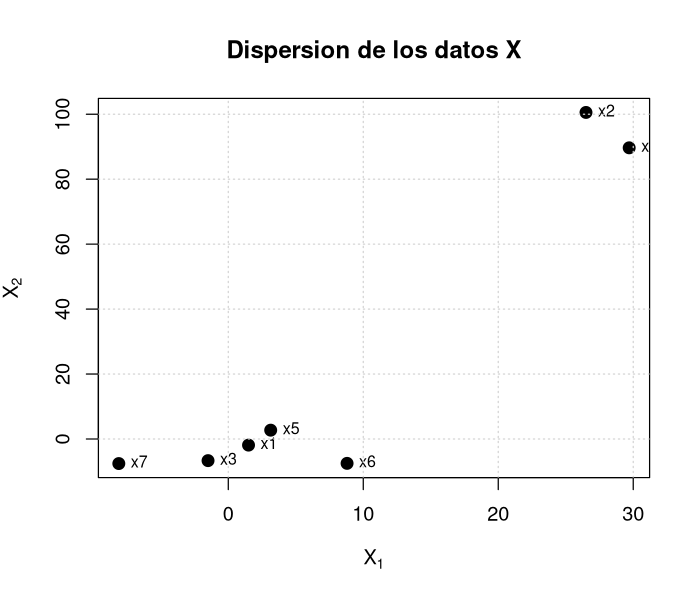
\includegraphics[width=0.75\textwidth]{dispersion.png}
  \caption{Gr\'afico de dispersi\'on de los 7 puntos $\mathbf{X} \in \mathbb{R}^2$.}
  \label{fig:dispersion}
\end{figure}

\begin{figure}[H]
  \centering
  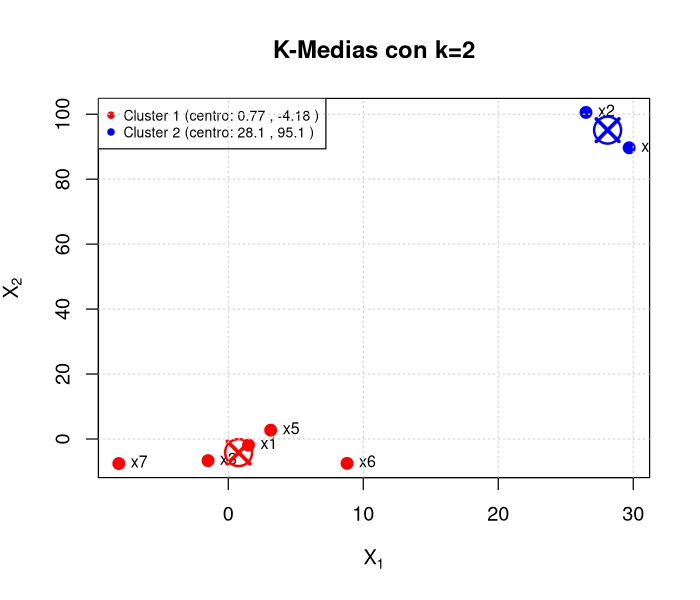
\includegraphics[width=0.75\textwidth]{kmeans_k2.png}
  \caption{K-medias con $k=2$. Los centros se marcan con $\times$.}
  \label{fig:k2}
\end{figure}

\begin{figure}[H]
  \centering
  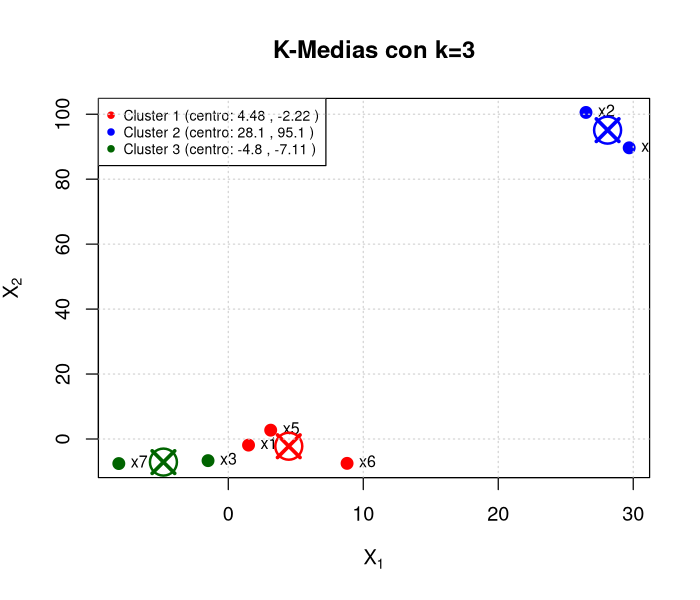
\includegraphics[width=0.75\textwidth]{kmeans_k3.png}
  \caption{K-medias con $k=3$. Los centros se marcan con $\times$.}
  \label{fig:k3}
\end{figure}

\subsection*{A.3 Bit\'acora de trabajo}

\begin{table}[H]
\centering
\footnotesize
\begin{tabular}{p{2.5cm} p{3cm} p{8cm}}
\toprule
\textbf{Fecha} & \textbf{Actividad} & \textbf{Descripci\'on} \\
\midrule
15/04/2026 & Lectura del enunciado & Comprensi\'on del problema y revisi\'on de diapositivas sobre k-medias (semana 5). \\
15/04/2026 & Desarrollo Pregunta 2 & Implementaci\'on del script R: dispersi\'on, k-medias $k=2$ y $k=3$, centroides. \\
15/04/2026 & Redacci\'on del informe & Elaboraci\'on del informe en \LaTeX{} seg\'un la pauta, integraci\'on de figuras y reflexi\'on. \\
\bottomrule
\end{tabular}
\caption{Bit\'acora de actividades del control.}
\end{table}

\end{document}
